\section{Evaluation}
\label{sec:eval}

We evaluate on a testbed with a physical master, one Tofino-1 switch, and a physical SEL-751 relay.
Native and defended traffic are captured on the same loaded program, separated only by a runtime mode
change, so the comparison isolates the defense. The defended captures carry no TCP timestamp option.
The analysis regenerates deterministically from the traces, and a manifest verifies every derived
artifact. Throughout, we separate what the hardware captures measure on the master-facing link from
what the offline model verifies and what is not observed.

\noindent\textbf{Timing (measured).} The native CLRT median is 1.272~ms for read (standard deviation
1.354, $n{=}999$) and 2.107~ms for select ($n{=}488$), with heavy tails. The defended CLRT median is
4.001~ms for both classes, with standard deviation 0.022 and 0.021~ms, matching the policy $R-A=4$~ms.
The master-facing offsets $A$ and $R$ measure about 21 and 25~ms, which include a documented path and
capture offset of roughly 1~ms over the configured 20 and 24~ms; the internal switch deadline was not
instrumented separately.

\noindent\textbf{Shape and reconstruction (measured).} The native read is one 49-byte segment. All
1{,}280 defended eligible responses (600 read, 500 select, and 90 select with 90 operate from the
control transactions) present the $[28,21]$ shape. Each is sequence-contiguous, valid under the DNP3
link and block CRCs, and valid under the IP and TCP checksums, and no defended response escapes as an
unsplit 49-byte segment. Because no paired source-side capture exists, we report a CRC- and
checksum-valid reconstruction, not byte identity to a source frame.

\noindent\textbf{Control-command timing (measured and modeled).} Fig.~\ref{fig:timeline} shows the
master-facing acknowledgment and echo of a control command. The echo-minus-acknowledgment gap is
4.00~ms and does not vary with the internal release delay: across the evaluated delays of 2, 6, and
12~ms the pooled gap median is 4.002~ms with standard deviation 0.026~ms ($n{=}90$). The relay-facing
release time and the number of copies delivered to the relay are not captured; the offline model
verifies the single release, and the captures establish that the master issued one OPERATE per
transaction.

\begin{figure}[t]
\centering
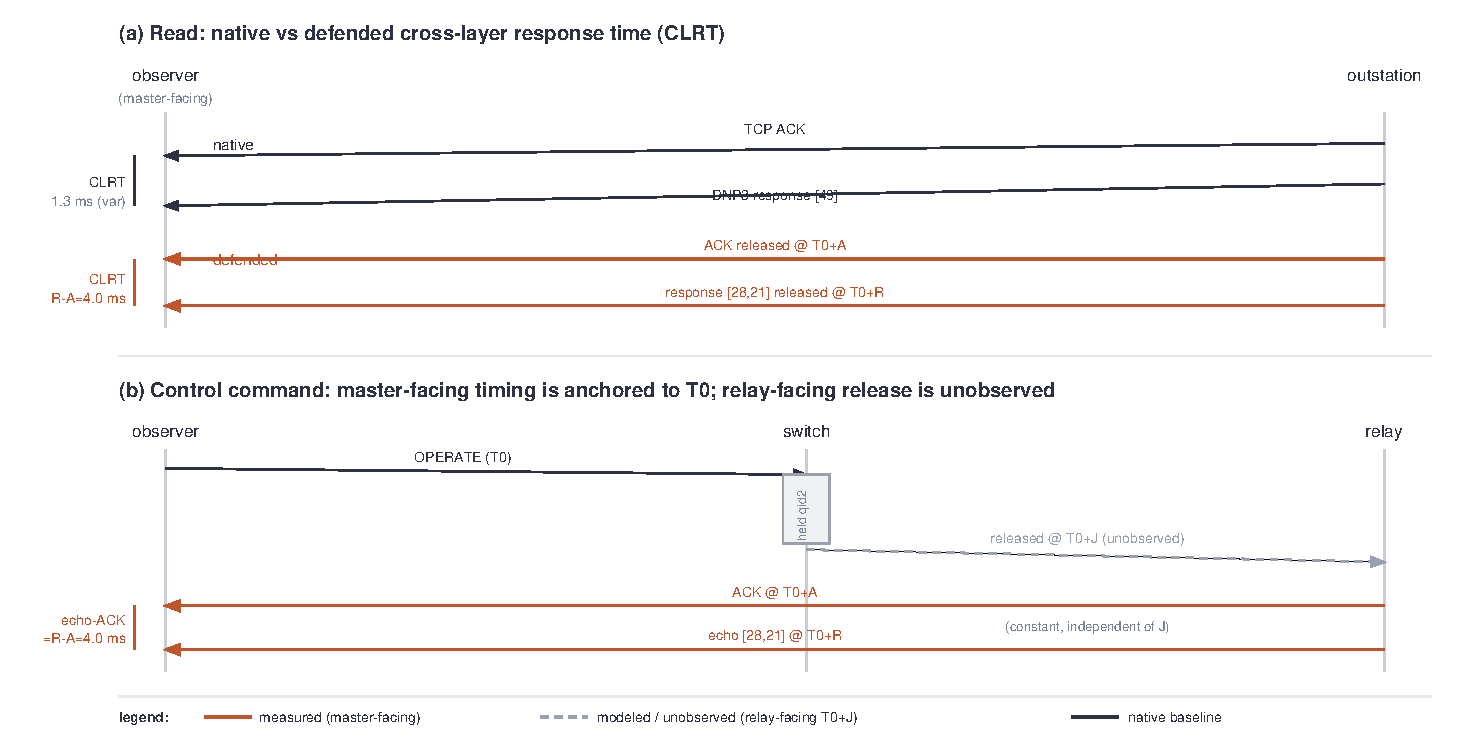
\includegraphics[width=0.98\columnwidth]{figures/fig_timeline}
\caption{Native versus defended timing, and the control-command timeline. The defended acknowledgment
and response are placed at $T_0{+}A$ and $T_0{+}R$; the internal release at $T_0{+}J$ is on the
relay-facing link and is not captured (dashed), so it is verified by the model rather than measured.}
\label{fig:timeline}
\end{figure}

\noindent\textbf{Fingerprint suppression (measured).} We quantify the leak with the mutual information
between the transaction class and the CLRT, using common bins and a permutation null. The native
mutual information is 0.424~bits, well above the null band, and the defended value is 0.0018~bits,
inside it. A logistic classifier trained to separate read from select by CLRT reaches 0.592 balanced
accuracy on native traffic and 0.500, the chance baseline, on defended traffic. This is a
transaction-class task on one device, not a device-identity task; the defense replaces the evaluated
CLRT and segment-shape features of this SEL-751 and does not establish indistinguishability among
devices.

\noindent\textbf{Safety and resource fit (measured).} The guarded control test permitted only two
isolated control points and refused the breaker-close point; all 32 relay outputs remained open
throughout, and no breaker operation was attempted. The program compiles for one ingress pipeline
within the twelve-stage budget.

\section{Discussion}
\label{sec:disc}

The defense replaces two master-facing features of one outstation with a fixed policy while preserving
the protocol. It does not hide the total 49-byte length, which a full TCP reader recovers, and it does
not establish indistinguishability among devices or resistance to every traffic-analysis feature.
Extending the eligible class beyond the 49-byte responses would require a segment-shape policy for each
response size; the CRC-block structure supports this, but we have not evaluated it. The strongest open
item is relay-facing verification: a tap on the relay-facing link would turn the modeled single
release into a measured property, and we leave that instrumentation to future work.
